\documentclass[12pt]{article}
% Эта строка — комментарий, она не будет показана в выходном файле
\usepackage{ucs}
\usepackage[warn]{mathtext}
\usepackage[utf8x]{inputenc} % Включаем поддержку UTF8
\usepackage[russian]{babel}  % Включаем пакет для поддержки русского языка
\usepackage{amsmath}
\usepackage{mathtools}
\usepackage{amssymb}
% \usepackage[dvips]{graphicx}
% \graphicspath{{noiseimages/}}
\usepackage[pdftex]{graphicx}


% Параметры страницы: 1см от правого края и 2см от остальных.


\hoffset=0mm
\voffset=0mm
\textwidth=180mm        % ширина текста
\oddsidemargin=-6.5mm   % левое поле 25.4 - 5.4 = 20 мм
\textheight=240mm       % высота текста 297 (A4) - 40
\topmargin=-15.4mm      % верхнее поле (10мм)
\headheight=5mm      % место для колонтитула
\headsep=5mm          % отступ после колонтитула
\footskip=8mm         % отступ до нижнего колонтитула


\begin{document}
    \author {Жарков Андрей 496}
    \title {Лабораторная работа 1.1 \\  Определение скорости полёта пули при помощи баллистического маятника}
    \maketitle{}
    
    \indent
    \textbf{Цель работы:} определить скорость полёта пули, применяя законы
    сохранения и используя баллистический маятник; познакомиться с
    базовыми принципами обработки экспериментальных данных.
    \\ \\
    \indent
    \textbf{В работе используются:} духовое ружье на штативе, осветитель, оптическая система для измерения отклонений маятника, измерительная линейка, пули и весы для их взвешивания, баллистический маятник.
    \\ \\
    
    Для измерения переданного пулей импульса и, следовательно, ее скорости используют баллистический маятник. Баллистическим называется маятник, колебания которого вызываются кратковременным начальным импульсом (толчком). Кратковременным можно считать импульс,
    если время действия сил (время соударения) значительно меньше периода колебаний маятника. При этом отклонение маятника за время
    соударения значительно меньше амплитуды колебаний — максимального отклонения маятника. \\
    
    \begin{center} 
    	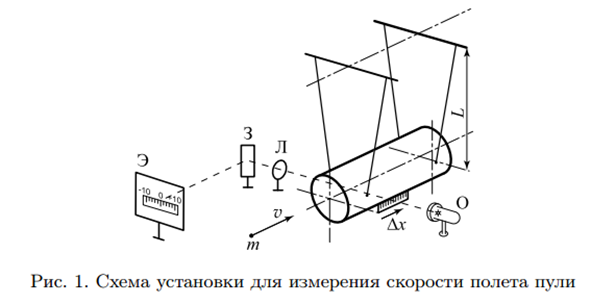
\includegraphics[width=5.5in]{lab1_1.png}
    \end{center}
    
    
    
    Используемый в этой работе баллистический маятник представляет
    собой тяжелый цилиндр, подвешенный на четырех нитях одинаковой
    длины. Он изображен на рис. 1 вместе с измерительной системой. Важной особенностью используемой системы подвески маятника является
    то, что при колебаниях ось цилиндра перемещается параллельно самой
    себе без вращения. Колебания происходят так, как будто вся масса маятника сосредоточена в его центре масс. Любая точка цилиндра при
    колебаниях маятника движется по дуге окружности, радиус которой
    равен расстоянию по вертикали между уровнями верхнего и нижнего
    концов нитей подвеса. \\
    
    Связь между максимальным отклонением маятника и начальной
    скоростью, полученной им в результате толчка, описывается законом
    сохранения механической энергии, если потери энергии за период значительно меньше энергии его колебаний. По начальному максимальному отклонению маятника определяются импульс и скорость пули. \\ 
    
    Внешними силами для системы пуля–цилиндр являются сила тяжести, которая не имеет горизонтальной компоненты, и силы натяжения
    нитей, у которых появляются горизонтальные компоненты при отклонении маятника. Однако если отклонения малы, то и эти компоненты
    малы. Тем более мал по сравнению с импульсом пули их импульс за
    время соударения. Поэтому закон сохранения импульса при соударении
    пули с цилиндром имеет вид 
    \begin{equation}
    	mu=(M+m)V
    \end{equation}
    Здесь 𝑚 — масса пули, 𝑀 — масса цилиндра, 𝑢 — скорость пули перед
    ударом, 𝑉 — скорость цилиндра и пули после неупругого соударения.
    Учитывая, что масса маятника значительно больше массы пули,
    можно написать
    \begin{equation}
    	u = \frac{M}{m}V
    \end{equation}
    Получив начальную кинетическую энергию, маятник при отклонении будет подниматься до тех пор, пока всю ее не израсходует. Если
    пренебречь потерями, то вся кинетическая энергия переходит в потенциальную в поле тяжести. Тогда по закону сохранения механической
    энергии высота ℎ подъема маятника над его начальным положением
    связана с начальной скоростью маятника 𝑉 следующим образом:
    \begin{equation}
    	V^2=2gh
    \end{equation}
    Высота подъема маятника выражается через угол $\phi$ отклонения маятника от вертикали:
    \begin{equation}
    	h = L(1-cos\phi)=2L\sin\frac{\pi}{2}^2, \mbox{ } где \phi = \frac{\Delta x}{L}
    \end{equation}
    
    Из (2), (3) и (4) получаем окончательную формулу для определения
    скорости пули ($\phi$ ≪ 1):
    \begin{equation}
        u = \frac{M}{m}\sqrt{\frac{g}{L}}\Delta x
    \end{equation}
    
    \pagebreak
    
    \textbf{\large Выполнение работы} \\ \\
     Параметры установки: \\
     $M = 2925 \pm 5 г.$ \\
     $L = 222 \pm 2 см.$ \\
     
     \begin{table}[ht]
     	\caption{измерения}
     	\begin{center}
     		\begin{tabular}{|c|c|c|c|c|c|c|c|c|}
     			\hline 
     			$i$ & 1 & 2 & 3 & 4 & 5 & 6 & 7 & 8 \\
     			\hline
     			$m$,мг & 516 & 513 & 523 & 528 & 518 & 520 & 520 & 521 \\
     			\hline
     			$\Delta x$, мм & 11.0 & 10.8 & 11.2 & 11.2 & 10.9 & 11.1 & 11.1 & 11.0 \\
     			\hline
     			$v$, м/с & 131.0 & 129.4 & 131.6 & 130.4 & 129.3 & 131.2 & 131.2 & 129.8 \\
     			\hline
     		\end{tabular}
     	\end{center}
     \end{table}
    
    $m_{ср} = 520 мг$ \\
    $\sigma_m = \sqrt{\frac{\Sigma (m_i - m_{cp})^2 }{n}}$ = 4.22мг 
     - среднеквадратичное отклонение от среднего\\
    $\sigma_{ср}=\frac{\sigma_m}{\sqrt{n}}=1.5мг$ \\ \\
    $\sigma_{суммы} = \sqrt{\Sigma \sigma_{m_i}^2} = 2.8мг$ \\
    $m_{совм} = 4.158 г$ \\
    $m_{суммы} = 4.1590 \pm 0.0028 г$ \\
    Совпаладают с учётом погрешности, аддитивность выполняется. \\ \\
    
    $\sigma_{\Delta x} \approx 0.3 мм$ (Вызвана начальными колебаниями системы и ценой деления) \\
    $\varepsilon_v = \sqrt{\varepsilon_M^2+\frac{1}{4}\varepsilon_L^2+\varepsilon_{\Delta x}^2 +
    	\varepsilon_m^2}$ = 2.7\%  \\
    $\sigma_v = v\varepsilon_v$ = 3.5 м/с \\
    \\
    $v_{ср} = 130.4$ м/с \\
    теперь среднеквадратичное отклонение \\
    $\sigma_v = \sqrt{\frac{\Sigma (v_i - v_{cp})^2 }{n}}$ = 0.83 м/с \\
    
    \textbf{\large Вывод} \\
      В погрешность измерения скорости наибольшее влияние оказало измерение $\Delta x$. Но даже так погрешность оказалась достаточно небольшой. Разброс скоростей связан с различными массами пуль.
    
\end{document}